\section{Auswertung}
\label{sec:Auswertung}
\subsection{Emissionsspektrum von Kupfer}
\label{subsec:spektrumCU}


In \autoref{fig:emissionssp} ist das Bremsspektrum der Röntgenstrahlung, die auf das Kupfer trifft, zu sehen.\\
Es wird die Zählrate $N$ der Impulse pro Sekunde gegen die Wellenlänge $\lambda$ in Metern aufgetragen.\\

\begin{figure}[H]
  \centering
  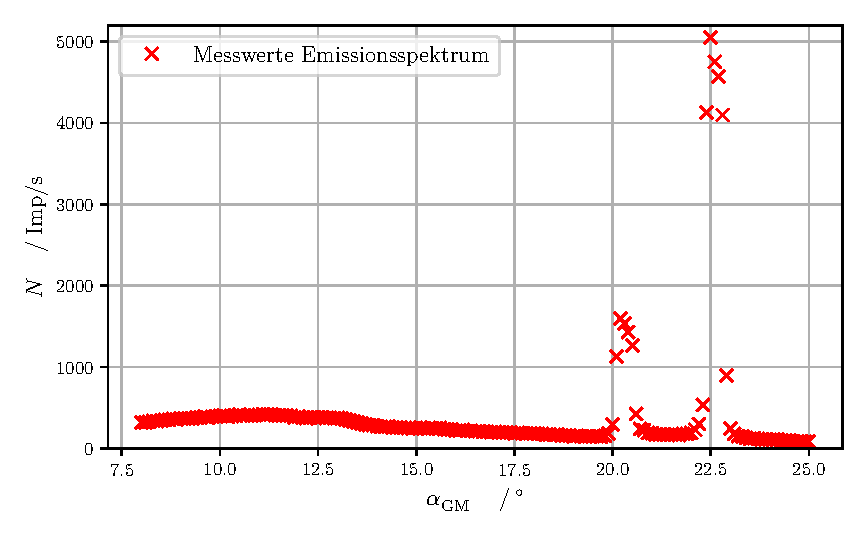
\includegraphics{build/emissionsspektrum.pdf}
  \caption{Das Emissionsspektrum von Kupfer mit gekennzeichneten Peaks. Der erste Peak stellt $K_{\beta}$ dar, der zweite $K_{\alpha}$.}
  \label{fig:emissionssp}
\end{figure}

\noindent Es sind die Peaks $K_{\alpha}$ und $K_{\beta}$ bei den Winkeln $\alpha(K_{\alpha})= \SI{22,5}{\degree}$ 
und $\alpha(K_{\beta}) = \SI{20,2}{\degree}$ zu erkennen.\\

\noindent Mit Hilfe der Formel
\begin{equation*}
  E = \frac{hc}{2d_{LiF}\sin\left(\alpha\right)}
\end{equation*}
nach Gl.\eqref{eqn:EHF} und Gl.\eqref{eqn:Bragg} lassen sich die zu den Peaks gehörigen Energien zu
\begin{align*}
  E(K_{\alpha}) &= \SI{8043,3545}{\electronvolt} \\
  E(K_{\beta}) &= \SI{8914,2038}{\electronvolt}
\end{align*}
bestimmen.




\subsection{Transmission $T$ des Aluminiumabsorbers}
\label{subsec:transmission}

Die Funktion der Transmisson $T(\lambda)$ beschreibt die Transmission der 
Röntgenstrahlung durch die Aluminiumplatte des Aufbaus in Abhängigkeit von der Wellenlänge.\\

\noindent Es wird die Totzeit $\tau$ des Geiger-Müller-Zählrohrs als $\tau = \SI{90}{\micro\second}$ angenommen. Die 
Integrationszeit der einzelnen Messungen lautet $t = \SI{200}{\second}$. \\
Die Wellenlängen $\lambda$ werden nach Gl.\eqref{eqn:Bragg} mit $n=1$, $d=d_{LiF}$ und den Winkeln $\alpha$ aus \autoref{tab:Tabelle1} bestimmt.
Die korrigierten Zählraten $I$ werden nach
\begin{equation*}
  I = \frac{N}{1-\tau N}
\end{equation*}
bestimmt und deren Fehler ergibt sich mit dem Fehler der Zählraten $\symup{\Delta}N = \sqrt{N}$ nach Gaußscher-Fehlerfortpflanzung zu
\begin{equation*}
  \symup{\Delta}I = \frac{\symup{\Delta}N}{\left(\SI{90e-6}{\second}\cdot N-1\right)^2}.
\end{equation*}
Der Fehler der Transmisson $T = \frac{I_{Al}}{I_0}$ wird nach
\begin{equation*}
  \symup{\Delta}T=\sqrt{\left(\frac{1}{I_0}\cdot\symup{\Delta}I_{Al}\right)^2+\left(-\frac{I_{Al}}{I_0^2}\cdot\symup{\Delta}I_{0}\right)^2}
\end{equation*}
bestimmt. Die Ergbnisse sind in \autoref{tab:Tabelle1} aufgeführt.
\begin{table}[H]
  \centering
  \caption{.}
  \begin{tabular}{ccccc}
    \toprule
    {$\alpha \mathbin{/} \unit{\degree}$} &
    {$\lambda \mathbin{/} \unit{\pico\meter}$} &
    {$I_0 \mathbin{/} \symup{Imp/s}$} &
    {$I_{Al} \mathbin{/} \symup{Imp/s}$} &
    {$T \mathbin{/} \symup{Imp/s}$} \\
    \midrule
    7.0 & 49.089 & 230.692 $\pm$ 1.108 & 114.671 $\pm$ 0.769 & 0.497 $\pm$ 0.004 \\
    7.1 & 49.787 & 236.947 $\pm$ 1.123 & 113.140 $\pm$ 0.764 & 0.477 $\pm$ 0.004 \\
    7.2 & 50.484 & 245.821 $\pm$ 1.146 & 113.140 $\pm$ 0.764 & 0.460 $\pm$ 0.004 \\
    7.3 & 51.118 & 253.662 $\pm$ 1.165 & 114.671 $\pm$ 0.769 & 0.452 $\pm$ 0.004 \\
    7.4 & 51.879 & 260.990 $\pm$ 1.183 & 116.203 $\pm$ 0.774 & 0.445 $\pm$ 0.004 \\
    7.5 & 52.576 & 268.327 $\pm$ 1.201 & 114.671 $\pm$ 0.769 & 0.427 $\pm$ 0.003 \\
    7.6 & 53.273 & 275.674 $\pm$ 1.218 & 114.161 $\pm$ 0.767 & 0.414 $\pm$ 0.003 \\
    7.7 & 53.970 & 283.030 $\pm$ 1.235 & 115.692 $\pm$ 0.772 & 0.409 $\pm$ 0.003 \\
    7.8 & 54.666 & 288.291 $\pm$ 1.248 & 115.182 $\pm$ 0.771 & 0.400 $\pm$ 0.003 \\
    7.9 & 55.363 & 297.245 $\pm$ 1.268 & 113.140 $\pm$ 0.761 & 0.381 $\pm$ 0.003 \\
    8.0 & 56.059 & 303.046 $\pm$ 1.282 & 110.590 $\pm$ 0.755 & 0.365 $\pm$ 0.003 \\
    8.1 & 56.755 & 308.325 $\pm$ 1.294 & 110.080 $\pm$ 0.753 & 0.357 $\pm$ 0.003 \\
    8.2 & 57.451 & 317.310 $\pm$ 1.314 & 109.060 $\pm$ 0.749 & 0.344 $\pm$ 0.003 \\
    8.3 & 58.147 & 319.956 $\pm$ 1.320 & 107.021 $\pm$ 0.742 & 0.334 $\pm$ 0.003 \\
    8.4 & 58.842 & 326.310 $\pm$ 1.334 & 105.492 $\pm$ 0.737 & 0.323 $\pm$ 0.003 \\
    8.5 & 59.538 & 333.732 $\pm$ 1.350 & 102.436 $\pm$ 0.726 & 0.307 $\pm$ 0.003 \\
    8.6 & 60.233 & 338.508 $\pm$ 1.361 & 100.908 $\pm$ 0.720 & 0.298 $\pm$ 0.002 \\
    8.7 & 60.928 & 342.757 $\pm$ 1.370 & 101.417 $\pm$ 0.722 & 0.296 $\pm$ 0.002 \\
    8.8 & 61.623 & 347.541 $\pm$ 1.381 & 98.363 $\pm$ 0.711 & 0.283 $\pm$ 0.002 \\
    8.9 & 62.317 & 351.265 $\pm$ 1.389 & 95.819 $\pm$ 0.701 & 0.273 $\pm$ 0.002 \\
    9.0 & 63.012 & 359.252 $\pm$ 1.406 & 93.277 $\pm$ 0.692 & 0.260 $\pm$ 0.002 \\
    9.1 & 63.706 & 361.384 $\pm$ 1.410 & 90.227 $\pm$ 0.680 & 0.250 $\pm$ 0.002 \\
    9.2 & 64.400 & 364.583 $\pm$ 1.417 & 88.703 $\pm$ 0.674 & 0.243 $\pm$ 0.002 \\
    9.3 & 65.094 & 368.317 $\pm$ 1.425 & 85.148 $\pm$ 0.660 & 0.231 $\pm$ 0.002 \\
    9.4 & 65.788 & 370.987 $\pm$ 1.431 & 83.625 $\pm$ 0.654 & 0.225 $\pm$ 0.002 \\
    9.5 & 66.481 & 375.794 $\pm$ 1.441 & 81.595 $\pm$ 0.646 & 0.217 $\pm$ 0.002 \\
    9.6 & 67.174 & 379.536 $\pm$ 1.449 & 79.059 $\pm$ 0.635 & 0.208 $\pm$ 0.002 \\
    9.7 & 67.868 & 381.675 $\pm$ 1.453 & 76.523 $\pm$ 0.625 & 0.200 $\pm$ 0.002 \\
    9.8 & 68.560 & 383.280 $\pm$ 1.457 & 74.496 $\pm$ 0.616 & 0.194 $\pm$ 0.002 \\
    9.9 & 69.253 & 388.098 $\pm$ 1.467 & 72.470 $\pm$ 0.608 & 0.187 $\pm$ 0.002 \\
    10.0 & 69.945 & 388.634 $\pm$ 1.468 & 68.925 $\pm$ 0.593 & 0.177 $\pm$ 0.002 \\
    \bottomrule
  \end{tabular}
  \label{tab:Tabelle1}
\end{table}

\begin{figure}[H]
  \centering
  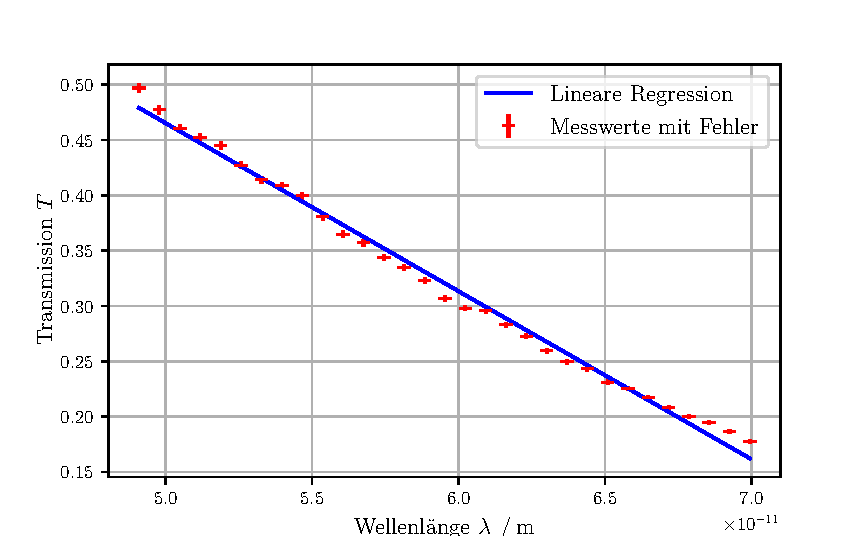
\includegraphics{build/transmission.pdf}
  \caption{Die Transmission $T$ in Abhängigkeit der Wellenlänge $\lambda$ mit linearer Ausgleichsgeraden.}
  \label{fig:transm}
\end{figure}

\noindent Die Ausgleichsgerade in \autoref{fig:transm} hat eine Gleichung der Form $T(\lambda) = a \cdot \lambda + b$ mit 
den Parametern $a = (-1,519 \pm 0,024)\cdot 10^{10}\symup{m}^{-1}$ und $b = 1,225 \pm 0,014$.

%\begin{figure}[H]
%  \centering
%  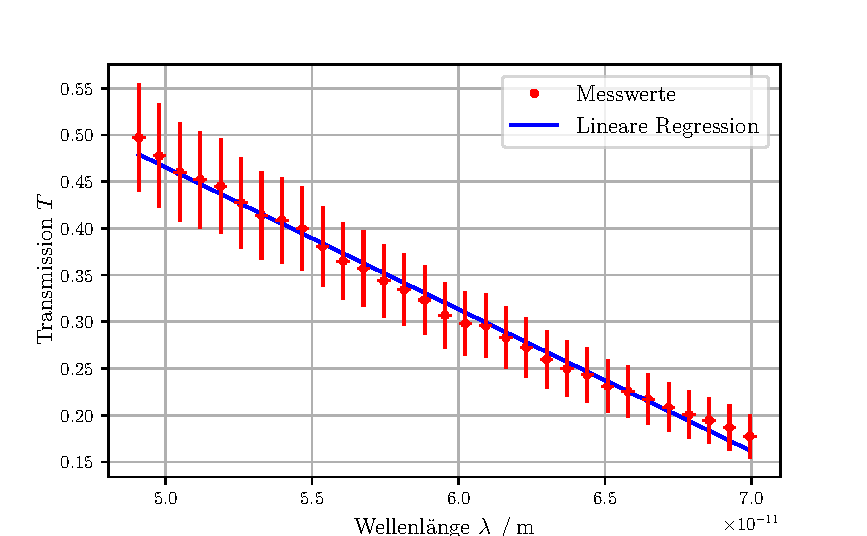
\includegraphics{build/transmission2.pdf}
%  \caption{Die Transmission $T$ in Abhängigkeit der Wellenlänge $\lambda$ mit linearer Ausgleichsgeraden und Fehlerbalken.}
%  \label{fig:transm2}
%\end{figure}



\subsection{Ermittlung der Compton-Wellenlänge}
\label{subsec:comptonwellenl}

Die Intensität $I_0 = 2731 \pm 50$ wird ohne Absorber, $I_1 = 1180 \pm 34$ und $I_2 = 1024 \pm 32$ mit Aluminiumabsorber zwischen Röntgenröhre
und Plexiglas-Streuer bzw. zwischen Plexiglas-Streuer und Geiger-Müller-Zählrohr gemessen.\\
Die dazugehörige Integrationszeit beträgt $t = \SI{300}{\second}$.\\

\noindent Aus den Intensitäten lassen sich die Transmissionen der Aufbauten mit $T_1 = \frac{I_1}{I_0}$ und $T_2 = \frac{I_2}{I_0}$ ermitteln. \\
Die Zählraten $N = \frac{I}{t}$ sind so klein das die Korrektur dieser nicht von nöten ist denn $1-\frac{N}{N_{korr}} < \SI{0,1}{\percent}$.\\
Die Transmissonen ergeben sich zu $T_1 = 0,423 \pm 0,015$ und $T_2 = 0,375 \pm 0,014$ und deren Fehler wurde nach
\begin{align*}
  \symup{\Delta}T_1 &= \sqrt{\left(\frac{1}{I_0}\cdot \symup{\Delta}I_1\right)^2 + \left(-\frac{I_1}{I_0^2}\cdot \symup{\Delta}I_0\right)^2} \\
  \symup{\Delta}T_2 &= \sqrt{\left(\frac{1}{I_0}\cdot \symup{\Delta}I_2\right)^2 + \left(-\frac{I_2}{I_0^2}\cdot \symup{\Delta}I_0\right)^2}
\end{align*}
ermittelt.\\

\noindent Schleißlich wird die Compton-Wellenlängen $\lambda_C$ aus den Transmissionen und den Parametern der Ausgleichsgerade 
in \autoref{fig:transm} bestimmt. \\
Mit 
\begin{align*}
  \lambda = \frac{T-b}{a}
\end{align*}
ergeben sich
\begin{align*}
  \lambda_1 &= (52,8 \pm 1,4) \cdot 10^{-12}\unit{\meter} \\
  \lambda_2 &= (56,0 \pm 1,3) \cdot 10^{-12}\unit{\meter},
\end{align*}
sodass die Compton-Wellenlänge sich auf $\lambda_C = \lambda_2 - \lambda_1 = (3,2 \pm 1,9) \cdot 10^{-12}\unit{\meter}$ beläuft.\\
Die Fehler der Wellenlängen $\lambda_1$ und $\lambda_2$ wurden nach
\begin{align*}
  \symup{\Delta}\lambda_1 &= \sqrt{\left(\frac{1}{a}\cdot \symup{\Delta}T_1\right)^2 + \left(-\frac{1}{a}\cdot \symup{\Delta}b\right)^2 + \left(-\frac{T_1-b}{a^2}\cdot \symup{\Delta}a\right)^2} \\
  \symup{\Delta}\lambda_2 &= \sqrt{\left(\frac{1}{a}\cdot \symup{\Delta}T_2\right)^2 + \left(-\frac{1}{a}\cdot \symup{\Delta}b\right)^2 + \left(-\frac{T_2-b}{a^2}\cdot \symup{\Delta}a\right)^2}
\end{align*}
bestimmt und der Fehler der Compton-Wellenlänge nach
\begin{equation*}
  \symup{\Delta}\lambda_C = \sqrt{\left(-\symup{\Delta}\lambda_1\right)^2 + \left(\symup{\Delta}\lambda_2\right)^2}
\end{equation*}
ermittelt.